The next tool that we will make is a proof of concept GUI that allows an end user to interface with the functionality
we have created by interacting with a user interface that we create.

For the website we will be relying on the plotly tool~\cite{plotlydash} as it is a relatively simple tool that will
allow us to quickly reach a minimum viable product

Our end goal for such a GUI would be to expose every functionality that the discovery tool provides, presented as a neat
visualisation that requires very little understanding of the underlying logic.
Once this is achieved, we can look into building more complex functionality that relies on the discovery tool.

\subsection{data input}\label{subsec:data-input}
The first and simplest step we have is to read the data from somewhere.
To do this we will simply create a folder on the filesystem that will be read from, we can then set up a callback
to periodically check if there have been updates to the folder, which will allow us to inject files from any source.

\begin{figure}[H]
    \centering
    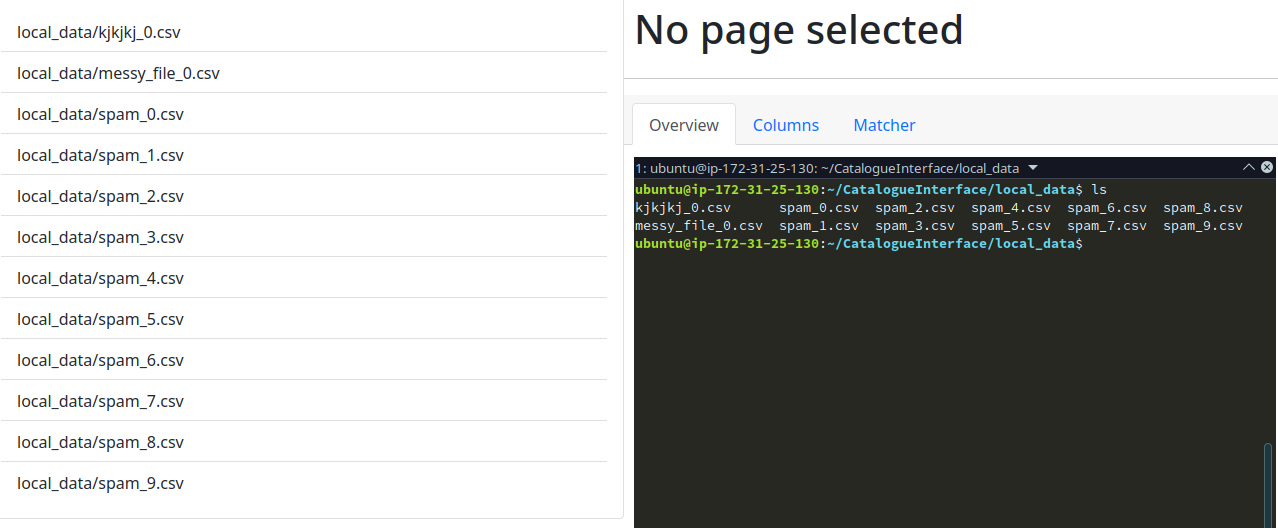
\includegraphics[width=12cm]{figures/website_images/website_data_catalogue}
    \caption{Demonstrating that the files in the data folder are being read}\label{fig:catalogue_file_list}
\end{figure}

\subsection{displaying metadata}\label{subsec:displaying-metadata}
When choosing a data file to look at, we would like to start by providing an overview of the file, giving surface level
information that a user can use to understand what they are looking at.
In our case we have chosen the pertinent information to be as follows:

- A list of tags assigned to the data file

- The file size and dimensions

- A snippet of the data file (such as displaying the first 10 rows)

- The ability to download the data file

\begin{figure}[H]
    \centering
    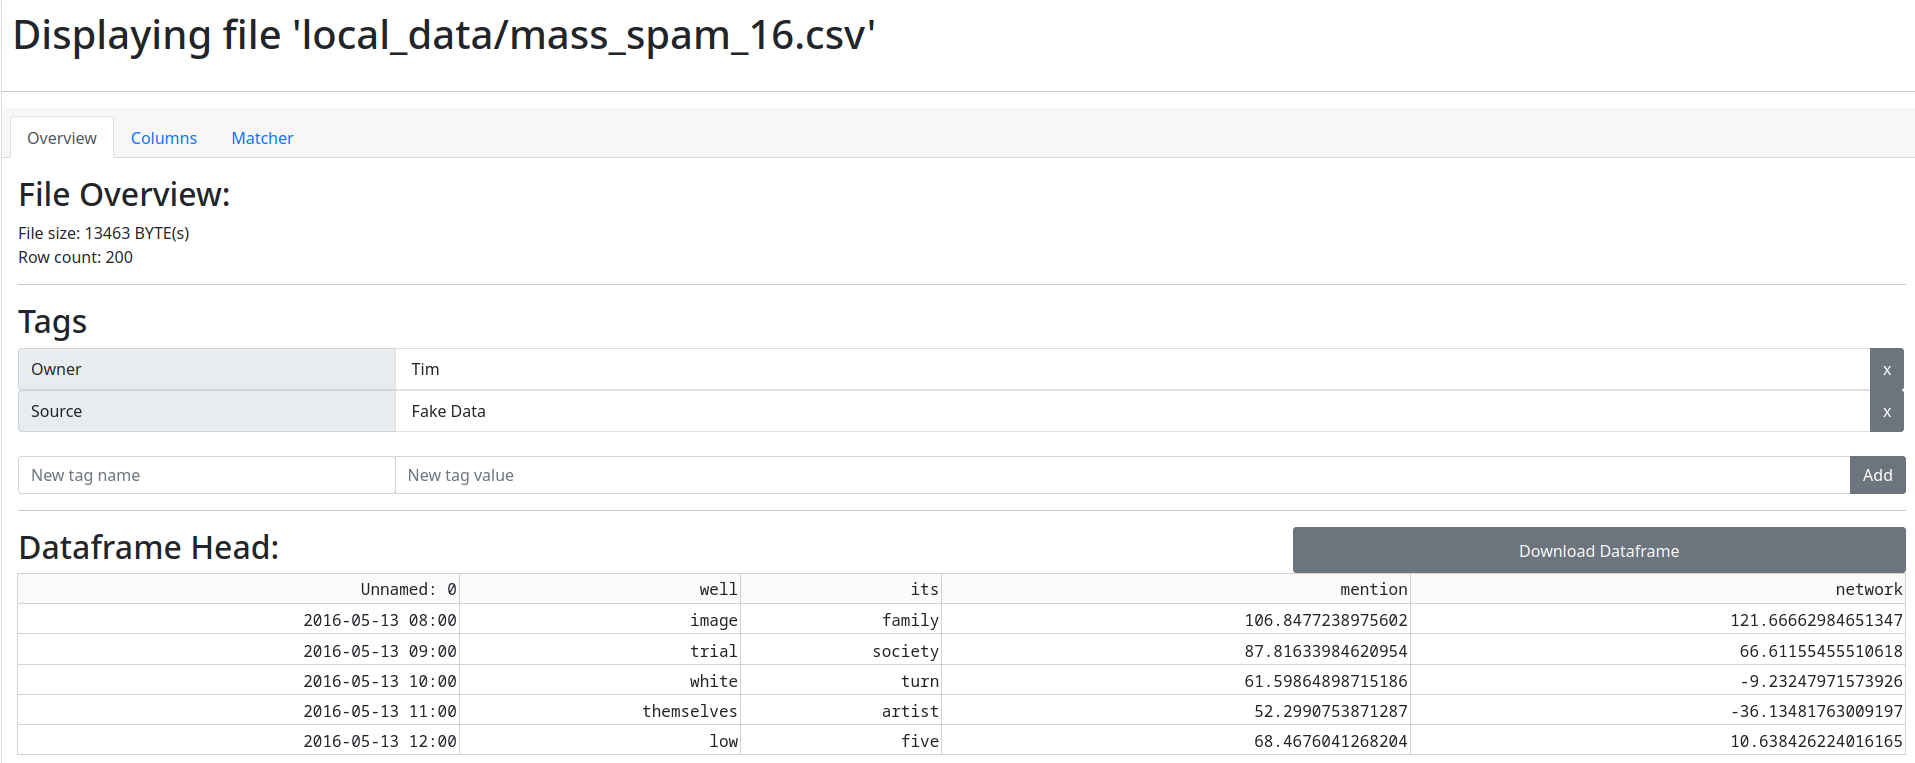
\includegraphics[width=12cm]{figures/website_images/catalogue_page_file_overview}
    \caption{Displaying an overview of the selected file}
    \label{fig:catalogue_file_overview}
\end{figure}

Our implementation, as pictured in ~\ref{fig:catalogue_file_overview} also includes the ability to add and remove
metadata tags.
Next, we display the individual columns and the metadata that is contained within them - this is demonstrated
in~\ref{fig:interface_column_values}.
As an additional quality of life feature we have colour coded relationship confidence, where 75\%+ is green, 50\%+ is
orange, and anything less is red.

\begin{figure}[H]
    \centering
    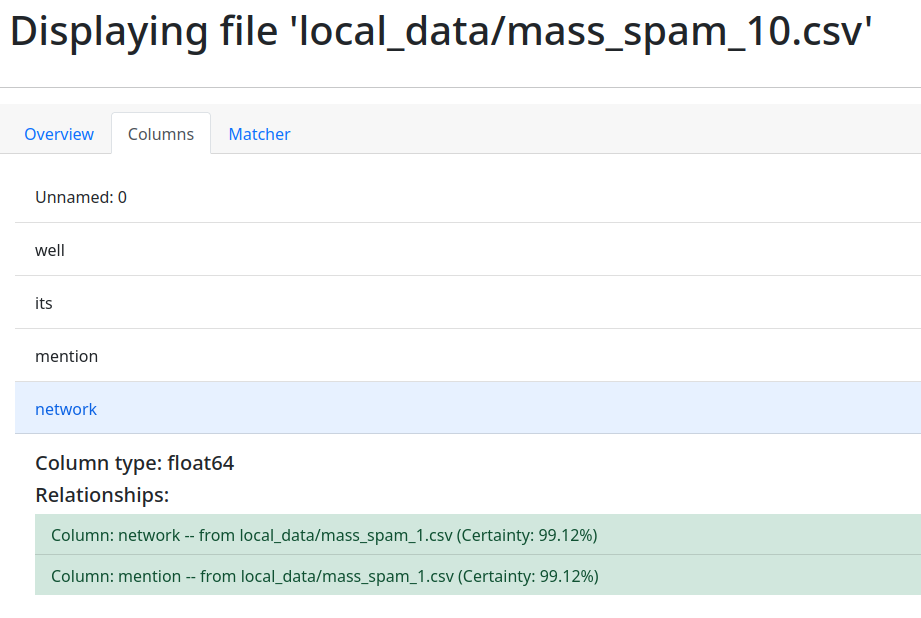
\includegraphics[width=12cm]{figures/website_images/interface_column_view}
    \caption{Displaying a single column within a metadata object}
    \label{fig:interface_column_values}
\end{figure}

\subsection{Reflection}\label{subsec:reflection}
In this section we have tried to avoid building new features that are not part of the discovery project itself, this has
resulted in a very sparse implementation of a user interface.
We believe, however, that we have successfully showcased the capabilities of our project as an approachable product.
In the future, we would consider building up functionality to complement the main project, creating a piece of
enterprise software that utilises it - rather than showcasing it.
